\chapter{Conclusion and Future Work}
\label{chp:6:ConcFutu}

\section{Conclusion}
\label{sec:6.1:Conc}

Increased Internet usage made email a popular medium for communication because of its low cost, quick turnover, and the flexibility of the connectivity via mobile devices. The benefits of email communication also attracted researchers to use it as a data collection method to explore, describe, and explain things via communicating large groups of people.
\vspace{1cm}

However, the nature of the communication with large groups is different than small ones due to the required effort to personalize messages according to the each recipient. As a result, researchers tend to write more generic emails, ignoring the recipient-specific details. Researchers investigated many response rate influences, and addressed that personalization of message content is an important factor to increase response rate \citep{Dillman1991,Schaefer1998}. The messages that are not personalized result in low response rate on the answers expected from the recipients. As a consequence, this may end up with a nonresponse error.
\vspace{1cm}

Nonresponse error has been considered a major problem by many researchers, because the characteristics of large groups of people who do not response might result in a biased estimate of representation of the population. Hence, it effects the outcome of a research \citep{Bogen1996}.
\vspace{1cm}

For this reason, researchers investigated the possible theories why personalization contribute on response rate. While \cite{DillmanDonA.SmythJoleneD.Christian2009} emphasized the social exchange theory since the personalization of emails helps to build a connection between the respondent and the researcher, \cite{Barron2002} stressed on the diffusion of responsibility theory in which being aware of other volunteers availability will result in a higher utility of not volunteering.
\vspace{1cm}

Researchers conducted studies investigate the diffusion of responsibility. \cite{Barron2002} showed that the proportion of replies where they used single email address in the "To" field got 20\% higher response and  the proportion of
"very helpful" replies was 187\% higher than the replies where they used groups of email addresses. In the study of \cite{Selm2006}, the recipients showed concerns regarding the confidentiality when the header of the email contained all the email addresses of the other respondents explicitly.
\vspace{1cm}

Some other researchers investigated the social exchange theory. \cite{Heerwegh2005} applied personalized salutations in the the emails, and got 6.9% higher
login rate to the provided survey link in the email than the unpersonalized group in their study. In the study of \cite{Joinson2007}, the power or status of the sender is combined with personalized status, they got 53.4\% response rate while non personalized salutation with neutral power of sender status got 40.1\% response rate.
\vspace{1cm}

Even though personalization of emails increases response rates, \cite{DillmanDonA.SmythJoleneD.Christian2009} emphasized on overwhelmed personalization that will still suffer of low response rates. Hence,  the adequate amount of personalization should be considered on personalized emails. In addition, the experienced email users can identify if a message is written by a person or computer generated easily. Therefore, the digital world make the true authentic personalization more rare, and achieving such a level of personalization requires getting to know each recipient very well.
\vspace{1cm}

To understand what do existing applications provide to support personalized mass email communication, the \ac{CRM}, the help desk, and the email marketing applications are evaluated in chapter \ref{chp:3:EvalExisAppl}. Several features of those applications are considered as a feature to that can help researchers on their mass email communication. Some of those features are followings:

\begin{compactitem}
	\item Keeping client related information extracted from conversations in \ac{KVP}s.
	\item Integration with popular email client such as Gmail.
	\item Importing recipients list from third part applications.
	\item Assigning emails to a recipient profile.
	\item Using dynamic variable in the emails to be replaced by their values.
	\item Assigning a help desk ticket to a assistant.
	\item Reusability of an existing email as a template.
\end{compactitem}
\vspace{1cm}

However, none of the available products offers all these mentioned features that might help a personalized mass email communication under one product, and some of those features also needs additional effort to use since their application area is not mass email communication. Therefore, this study came up with an initial solution as a prototype in chapter \ref{chp:4:InitIdeaProt}. The prototype supported following features to help a researcher to reach a large groups of people in a personalized way with less effort:

\begin{compactitem}
	\item Kept extracted information in \ac{KVP}s along with the recipient messages.
	\item Used dynamic variables to personalize the salutations of emails.
	\item Allowed to reuse earlier send messages as a template.
	\item Provided a tree structure to visualize the state of the conversation with the used templates.
\end{compactitem}
\vspace{1cm}

Even though, the prototype provided the above mentioned features to support a personalized mass email communication, we moved the prototype from its origin product, EmailValet to a new project after the informal user test with an organization who does mass email communication regularly at Stanford. The user test ended up with new features, and made us realize the drawbacks of existing EmailValet as a email client that we used in the prototype.
\vspace{1cm}

The improved requirements after user test brought up the final solution in chapter \ref{chp:5:FinaSolu}, and its features to support mass email communication as follows:

\begin{compactitem}
	\item Recipients information can be synchronized to the Myriad via Google Spreadsheet to remove the effort on importing and exporting recipients information from researchers.
	\item A researcher can assign assistants to an email campaign to interact the flow of a mass email communication with tasks such as extracting information from the incoming answers, proofreading the primary researcher's replies before sending, or even writing replies to those answers.
	\item Extracted respondents information can be recorded to recipients' profiles in \ac{KVP}s during the whole state of a campaign. 
	\item Those recorded \ac{KVP}s can be used as dynamic variables to personalize the content of the emails.
	\item Reusability of exiting emails, and visualizing the state of the conversation.
	\item Provided decision-making mechanism to automate earlier decisions on sending emails in a user verified manner.
	\item Provided visual cues to notify users what is the state of communication with individual recipients, and suggesting potential action according to the previous decisions of the user.
	\item Each recipient's all conversations and extracted information are provided under one view to conveniently reach all the necessary information to write recipient specific personalize emails.
 \end{compactitem}

Considering the features gathered in the final solution, we provided a workflow to researchers reducing the amount of time to personalize the content of the emails. If we take the Effort vs Personalization chart from figure \ref{fig:ChartEffortCustom} into consideration again after the final solution, it could be replaced as in the figure \ref{fig:drawingEfforPersonalizationAnnotations} compared with other products in the market focusing on email communication and data collection. Considering the user feedbacks, and the amount of people that already actively using Myriad in its beta stage, we believe that Myriad becomes more closer to the gold standard of effort vs. personalization that annotated in the figure.
\vspace{1cm}

However, there are possible future work that can enhance existing solution to a better state, and remove existing restrictions as we will discuss in the next section.
\clearpage 

\begin{figure}[htbp]
	\centering
	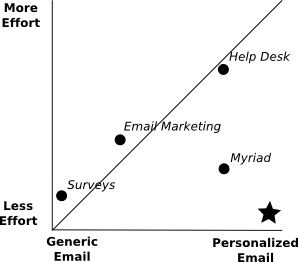
\includegraphics[width=.55\textwidth]{imgs/drawingEfforPersonalizationAnnotations.png}
	\caption[Effort vs Personalization and the Comparison of Available Solutions]{Effort vs Personalization and the Comparison of Available Solutions}
	\label{fig:drawingEfforPersonalizationAnnotations}
\end{figure}

\section{Future Work}
\label{sec:6.2:FutuWork}

The provided assistant support in the final solution helps researchers to share the tasks to extract information from emails, to proofread the primary researcher's replies before sending, to write replies to recipients' emails, and to verify the rule-based actions before taken.
\vspace{1cm}

Along with the assistant support, the system could provide an option in which crowd of anonymous workers can do the tasks of assigned assistants as a crowd assistant. If the system provides the required functionality to involve crowd assistants, the decisions on the possible tasks in a mass email communication can be done by anonymous crowed workers.
\vspace{1cm}

\cite{Surowiecki2005} stated that under the right conditions, groups can be remarkably smart, and even smarter than the smartest person within them. Therefore, if you try to solve a complicated problem or try to make a decision, the best thing that can be done
is to ask a group instead of trying to find an expert. Therefore, leveraging crowed assistants can minimize the work that a researcher need to do at a personalized mass email communication.

Another 


 